%!TeX root=../tese.tex
%("dica" para o editor de texto: este arquivo é parte de um documento maior)
% para saber mais: https://tex.stackexchange.com/q/78101/183146

%% ------------------------------------------------------------------------- %%
\chapter{Conceitos}
\label{cap:concepts}

Este capítulo visa apresentar os conceitos que foram utilizados para o desenvolvimento deste TCC. Serão apresentadas as ferramentas utilizadas para realizar o ETL, simular os logs de ataques, modelos que foram utilizados e por fim quais frameworks usados para o aprendizado de máquina.

\section{Ferramentas}

\begin{description}
    \item[Kali Linux] \hfill \\ 
        O Kali Linux é uma distribuição linux open source baseada em Debian. Tem como foco auxiliar em tarefas relacionada a segurança da informação e testes de penetração.
    \item[xsser] \hfill \\ 
        O xsser é um utilitário que está instalado por padrão no kali linux. Sua função é automatizar a deteccão, exploração e análise de ataques XSS em aplicações web.
    \item[sqlmap] \hfill \\ 
        O sqlmap é um utilitário que vem está instalado por padrão no kali linux. Sua função é automatizar a detecção e exploração de ataque de SQL injection em aplicações web.
    \item[Pandas] \hfill \\ 
        O Pandas é uma ferramenta  em python para o processo de análise de dados, especificamente neste trabalho, foi utilizado para realizar o ETL e analise dos logs coletados.
    \item[DVWA] \hfill \\ 
        DVWA é uma aplicação web com falhas de segurança conhecidas que podem ser exploradas no ambiente local e controlado.
  \end{description}

\section{Modelos}


\begin{description}
    \item[Árvore de decisão] \hfill \\ Árvore de decisão é um modelo de representação dos dados que, neste trabalho, visa classificar os dados tendo como base um conjunto de atributos. \\ 
    Elas são construidas particionando os dados em conjuntos, chamados de nós, até que uma folha seja encontrada, está então é a classe do dados. Veja na imagem abaixo.
    
    \begin{figure}
        \centering
        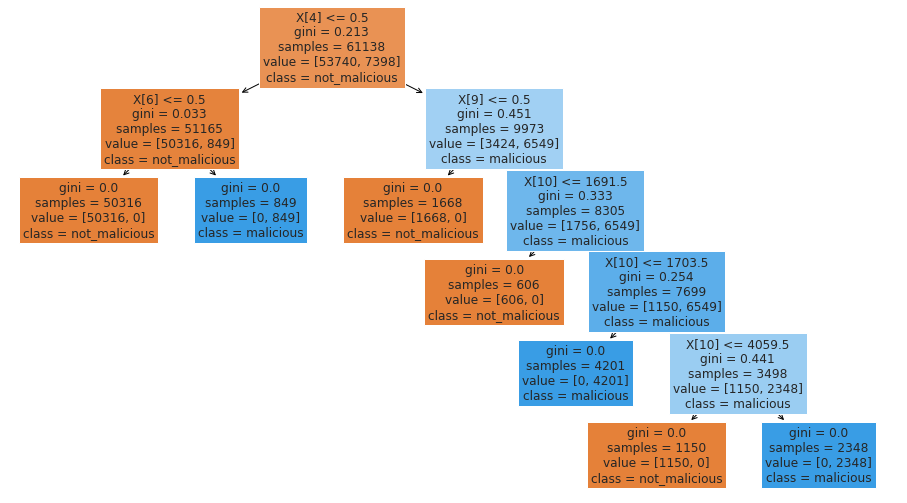
\includegraphics[width=.6\textwidth]{figuras/ex_decicion_tree.png}
        \caption{Exemplo de árvore de decisão.\label{fig:ex_decision_tree}}    
    \end{figure}

    Este modelo é útil pois a sua interpretabilidade é alta.

    \item[Florestas aleatórias] \hfill \\ Florestas aleatórias é um modele de aprendizagem de máquina de combina árvores de decisão. Isto é, uma certa quantidade de árvores são treinadas independetes uma das outras, utilizando diferentes partes do conjunto de dados. \\ 
    E para realizar a classificação, cada árvore realiza uma classificação (voto) e o resultado final da floresta é a classe com mais votos, como ilustrado na image abaixo:\\

    \begin{figure}
        \centering
        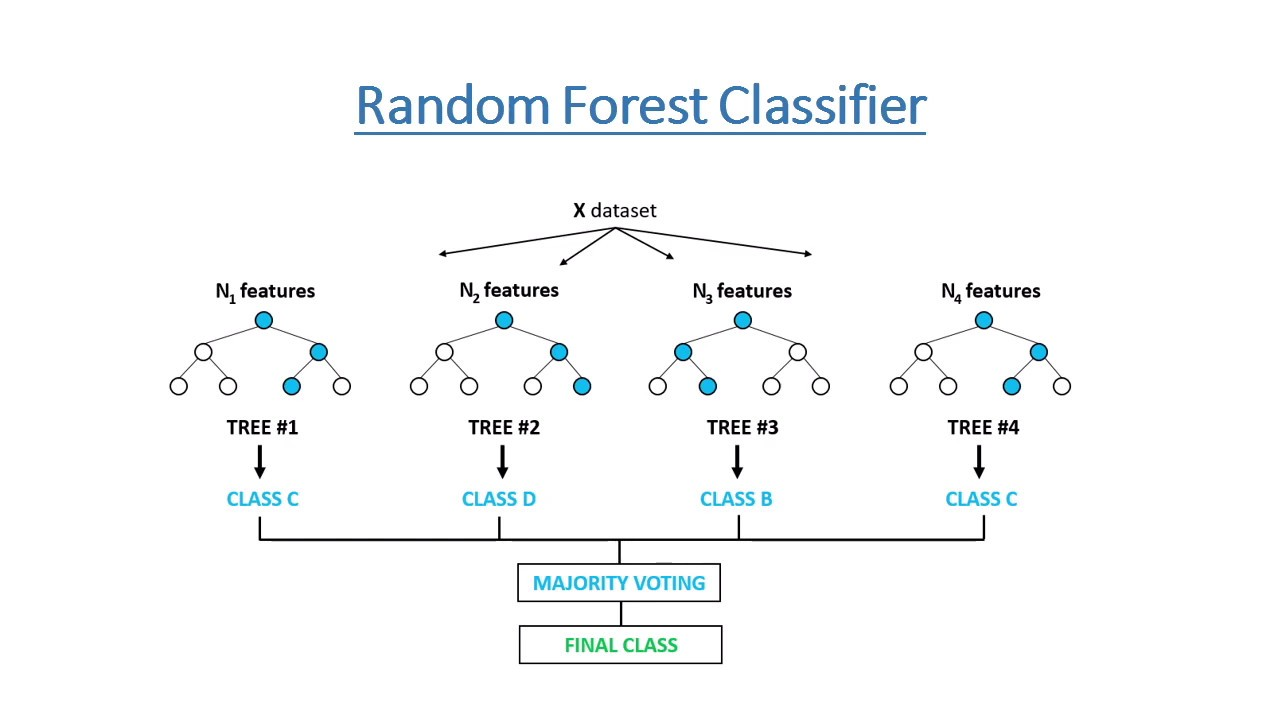
\includegraphics[width=.8\textwidth]{figuras/ex_random_forest.jpg}
        \caption{Exemplo de floresta aleatória.\label{fig:ex_random_forest}}    
    \end{figure}

    Este modelo possui dois pontos de atenção: sua interpretabilidade é baixa, dado o número de classificadores que temos que analisar, e também é consideravelmente mais pesado que o anterior, pois ele treina algumas árvores de decisão.
\end{description}

\section{Ferramentas de aprendizado de máquina}

\begin{description}
    \item[scikit-learn] \hfill \\ Scikit-learn é uma ferramenta que implementa algoritmos de aprendizagem de máquina, supervisionados e não supervisionados. Em particular, o modelo de árvore de decisão e floresta aletória.\\ 
    Além disso, ela integra com o ecossistema python, isto é: numpy, pandas e matplotlib. Além de fornecer uma interface sólida, que facilita o seu uso. 

    \item[Apache Spark] \hfill \\ Apache Spark é uma ferramenta para trabalhar com aprendizagem de máquina de maneira distribuida ou em um único nó. \\
    Assim como o scikit-learn, há alguns modelos implementados que estão pronto para ser utilizados, em particular, há implementações de árvore de decisão e floresta aleatória. \\
    Há suporte para algumas linguagens, como: Python, Scala, Java e R.
\end{description}